\section*{Risultati}
I risultati ottenuti in questo esperimento sono esposti rispettivamente per ogni sostanza adoperata. 
Per ciascuna sostanza sono stati tracciati grafici e acquisiti dati provenienti da diverse configurazioni per il software UPENWin. 

Le configurazione usate sono state oltre a quella di default:  - l'uso del doppio dei dati per l'inversione; - la variazione del parametro di smoothing, che è stato adoperato per l'analisi in undersmoothing a valori 5 e 10.
In particolare queste configurazioni sono state definite rispettivamente su: - ciascun $\tau$; - i due $\tau$ maggiori.

Non è stato ritenuto significativo tener conto dell'analisi in oversmoothing poichè per tutte le sostanze le curve delineate mostrano la presenza nitida di un solo picco.
Ciò è confermato anche dai grafici (non riportati) relativi all'undersmoothing.

Lo stesso procedimento è stato adottato per ogni sostanza ed in particolare il valore dei tempi $T_2$ è stato considerato come il punto con massimo segnale nella curva; mentre l'incertezza associata è stata calcolata come la differenza tra i primi due punti simmetrici dopo il picco.

\subsection*{$H_2O$}
La prima sostanza esaminata è stata una soluzione composta principalmente d'acqua e con una piccola percentuale di rame e di sale EDTA.
Sono stati elaborati i dati attraverso il software UPENWin per ottenere la distribuzione dei tempi di rilassamento trasversali per $\tau$ (metà del tempo di eco) uguale a 25, 35, 50, 75, 100 e 175 ${\mu}s$.

Sono riportate di seguito(tabella \ref{tab:T_h2o}) i tempi ricavati con le relative incertezze, i quali sono stati rispettivamente calcolati come la media tra le varie configurazioni e come la massima larghezza tra i primi due punti simmetri dopo il picco.

\begin{table}
    \begin{center}
    \begin{tabular}{c c c}
    \toprule
    	${\tau}\,({\mu}s)$ & $T\,(ms)$ & ${\sigma}\,(ms)$ \\
    \midrule
	25 & 79 & 9 \\
	35 & 45 & 18 \\
	50 & 23 & 8 \\
	75 & 10 & 3 \\
	100 & 6 & 3 \\
	175 & 2.6 & 1.9\\
    \bottomrule
    \end{tabular}
    \caption{Tempi di rilassamento trasversale relativi ai diversi tempi $\tau$.}
    \label{tab:T_h2o}
    \end{center}
\end{table}

Sono stati tracciati i grafici \ref{fig:D_h2o} e \ref{fig:S_h2o} relativi alle distribuzioni dei tempi di rilassamento e all'intensità dei segnali acquisiti per l'acqua nella configurazione in cui UPEN calcola il doppio dei punti d'inversione, ritenuta la più rappresentativa.

\begin{figure}[p]
\centering
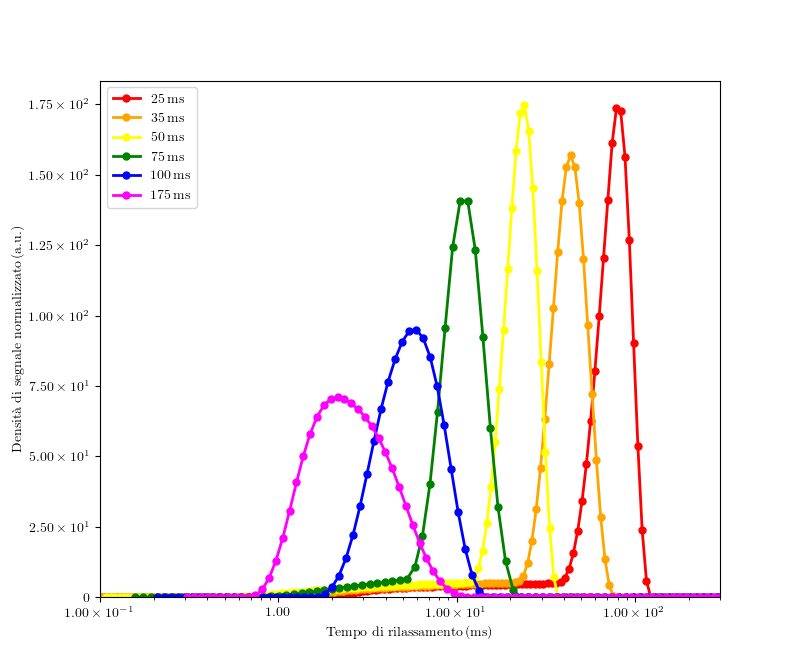
\includegraphics[width=\columnwidth]{Figure/H2O.png}
\caption{Distribuzioni dei tempi di rilassamento dell'acqua per ciascun $\tau$.}
\label{fig:D_h2o}
\end{figure}

\begin{figure}[p]
\centering
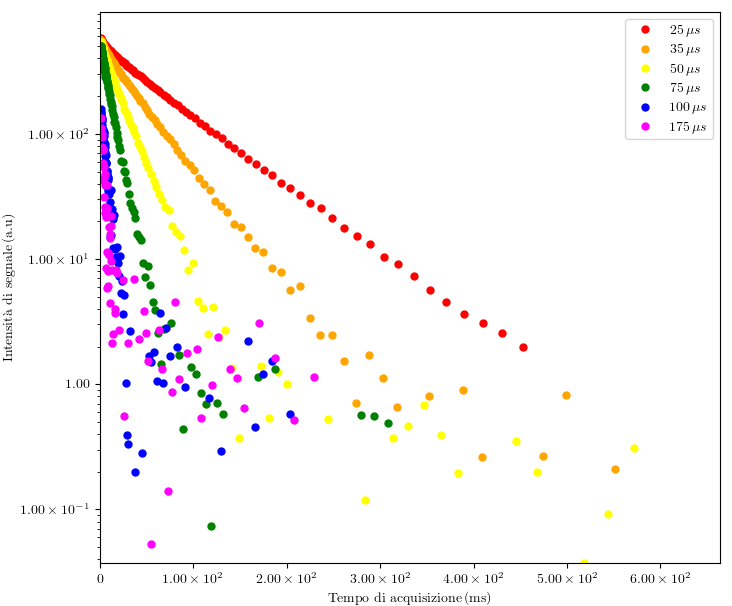
\includegraphics[width=\columnwidth]{Figure/H2O_SigTSig.png}
\caption{Intensità dei segnali dell'acqua per ciascun $\tau$.}
\label{fig:S_h2o}
\end{figure}
\newpage
In seguito è stato calcolato analiticamente il coefficiente di autodiffusione a partire da una regressione lineare pesata eseguita sui dati di tabella \ref{tab:T_h2o}.
Il grafico seguente \ref{fig:Df_h2o} riporta l'andamento di tale fit.

\begin{figure}[p]
\centering
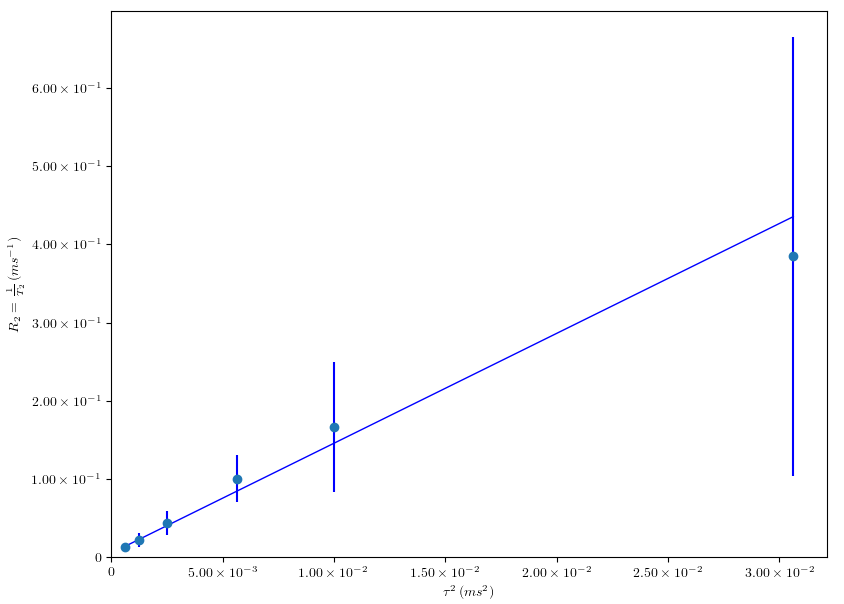
\includegraphics[width=\columnwidth]{Figure/H2O_calc.png}
\caption{Fit dei dati ottenuti per l'acqua.}
\label{fig:Df_h2o}
\end{figure}
\newpage
Il risultato finale per il coefficiente di autodiffusione associato all'errore è riportato nella tabella seguente.

\begin{table}
    \begin{center}
    \begin{tabular}{c c c}
    \toprule
    	$D\,(\frac{{\mu}^2}{ms})$ & $\sigma\,(\frac{{\mu}^2}{ms})$ \\
    \midrule
    	2.04	&	0.16	\\
    \bottomrule
    \end{tabular}
    \caption{Coefficiente di autodiffusione dell'acqua con relativo errore.}
    \label{tab:Df_h2o}
    \end{center}
\end{table}


\subsection*{SOLTROL 130}

La seconda sostanza considerata è stata il soltrol 130.
Come per l'acqua, tramite il software UPENWin sono state delineate le distribuzioni dei tempi di rilassamento trasversali per $\tau$ (metà del tempo di eco) uguali a 20, 25, 30, 40, 50, 70, 90, 100 ${\mu}s$.

Sono riportate in tabella \ref{tab:T_s130} i tempi ottenuti con le relative incertezze, calcolate secondo lo stesso metodo applicato per l'acqua.

\begin{table}
    \begin{center}
    \begin{tabular}{c c c}
    \toprule
    	${\tau}\,({\mu}s)$ & $T\,(ms)$ & ${\sigma}\,(ms)$ \\
    \midrule
	 20 & 150 & 40 \\
	 25 & 120 & 30 \\
	 30 & 100 & 20 \\
	 40 & 67 & 16 \\
	 50 & 47 & 12 \\
	 70 & 27 & 6 \\
	 90 & 18 & 5 \\
	 100 & 15 & 4 \\
    \bottomrule
    \end{tabular}
    \caption{Tempi di rilassamento trasversale relativi ai diversi tempi $\tau$ per il soltrol 130.}
    \label{tab:T_s130}
    \end{center}
\end{table}
\newpage
Sono stati poi descritti i grafici \ref{fig:D_s130} e \ref{fig:S_s130} che rappresentano le distribuzioni dei tempi di rilassamento e l'intensità dei segnali acquisiti per il soltrol 130 nella configurazione in cui UPENWin calcola il doppio dei punti d'inversione, ritenuta la più rappresentativa.

\begin{figure}[p]
\centering
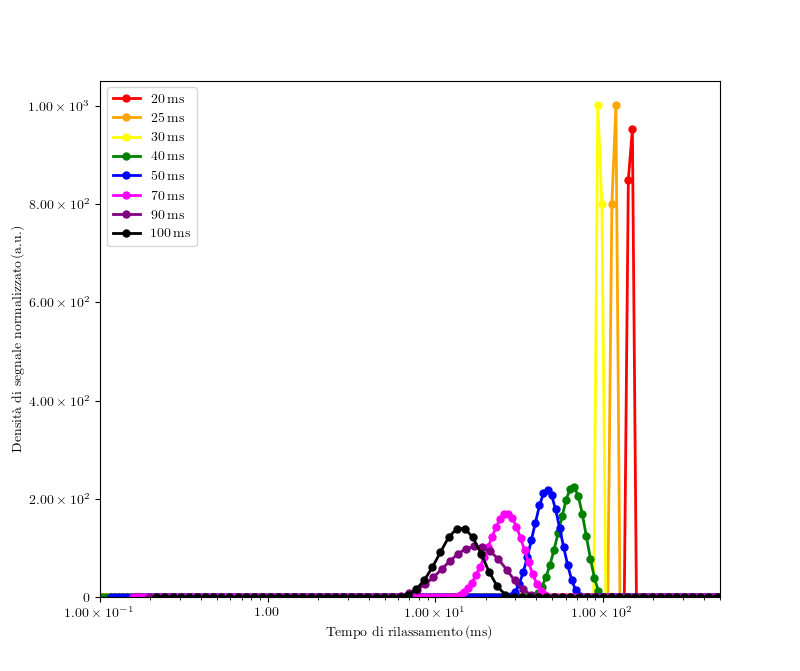
\includegraphics[width=\columnwidth]{Figure/SOLTROL130.png}
\caption{Distribuzioni dei tempi di rilassamento del soltrol 130 per ciascun $\tau$.}
\label{fig:D_s130}
\end{figure}

\begin{figure}[p]
\centering
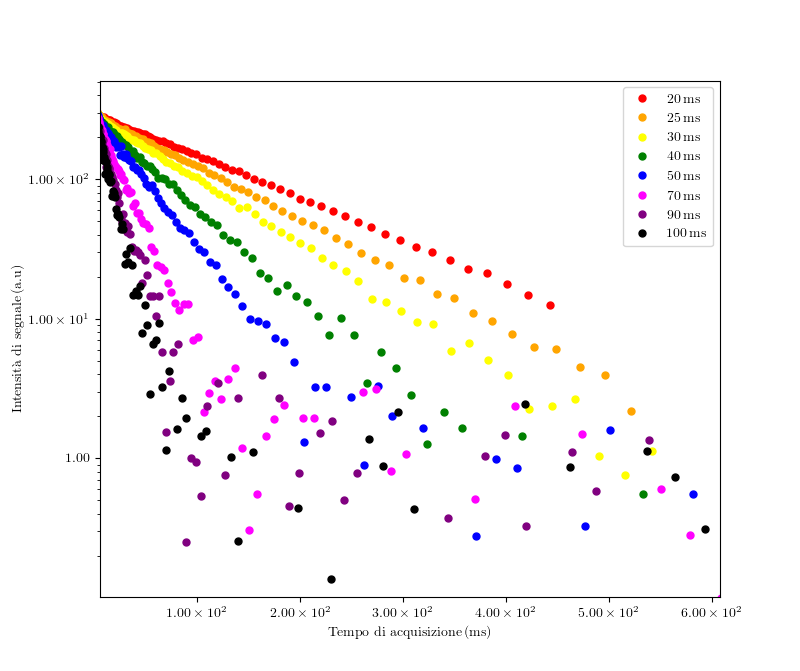
\includegraphics[width=\columnwidth]{Figure/SOLTROL130_SigTSig.png}
\caption{Intensità dei segnali del soltrol 130 per ciascun $\tau$.}
\label{fig:S_s130}
\end{figure}
\newpage
\'E stato poi ottenuto il coefficiente di autodiffusione usando inizialmente una regressione lineare pesata eseguita sui dati di tabella \ref{tab:T_s130}, come proceduto per l'acqua.
Il grafico seguente \ref{fig:Df_s130} riporta l'andamento di tale fit.

\begin{figure}[p]
\centering
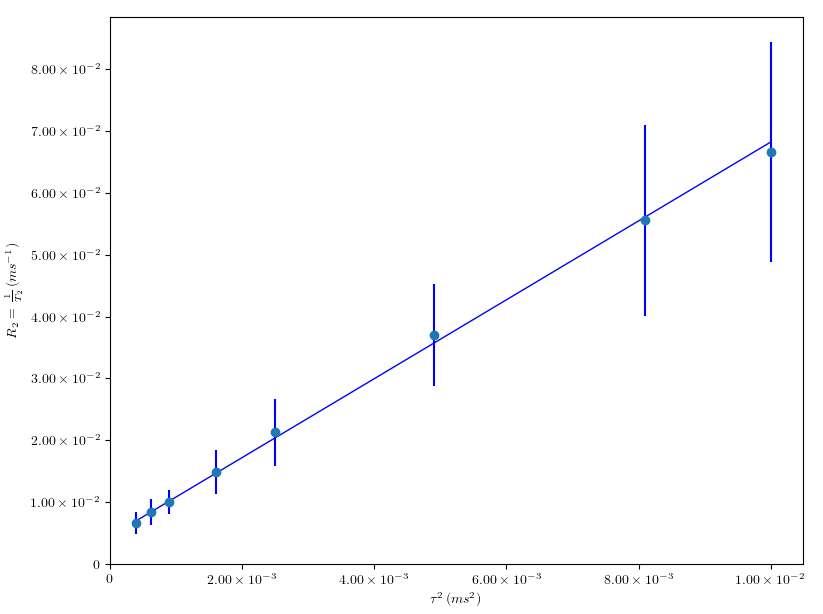
\includegraphics[width=\columnwidth]{Figure/SOLTROL130_calc.png}
\caption{Fit dei dati ottenuti per il soltrol 130.}
\label{fig:Df_s130}
\end{figure}

Il risultato finale per il coefficiente di autodiffusione del soltrol 130 assieme alla sua incertezza è riportato nella tabella seguente.

\begin{table}
    \begin{center}
    \begin{tabular}{c c c}
    \toprule
    	$D\,(\frac{{\mu}^2}{ms})$ & $\sigma\,(\frac{{\mu}^2}{ms})$ \\
    \midrule
    	0.927	&	0.015	\\
    \bottomrule
    \end{tabular}
    \caption{Coefficiente di autodiffusione del soltrol 130 con relativo errore.}
    \label{tab:Df_s130}
    \end{center}
\end{table}


\subsection*{SOLTROL 170}

L'ultima sostanza analizzatat è stata il soltrol 170.
Analogamente a come è stato eseguito per l'acqua e il soltrol 130, il software UPENWin è stato adoperato per descrivere le distribuzioni dei tempi di rilassamento trasversali per $\tau$ (metà del tempo di eco) pari a 25, 50, 75, 100, 125, 150 ${\mu}s$.

Nella tabella seguente \ref{tab:T_s170} sono riportati i tempi calcolati assieme all'errore associato, ricavati come citato in precedenza.

\begin{table}
    \begin{center}
    \begin{tabular}{c c c}
    \toprule
    	${\tau}\,({\mu}s)$ & $T\,(ms)$ & ${\sigma}\,(ms)$ \\
    \midrule
	 25 & 200 & 50 \\
	 50 & 100 & 30 \\
	 75 & 51 & 12 \\
	 100 & 33 & 7 \\
	 125 & 21 & 5 \\
	 150 & 14 & 3 \\
    \bottomrule
    \end{tabular}
    \caption{Tempi di rilassamento trasversale relativi ai diversi tempi $\tau$ per il soltrol 170.}
    \label{tab:T_s170}
    \end{center}
\end{table}

I grafici seguenti \ref{fig:D_s170} e \ref{fig:S_s170} mostrano le distribuzioni dei tempi di rilassamento e l'intensità dei segnali acquisiti per il soltrol 170 nella configurazione rappresentativa, in cui UPENWin calcola il doppio dei punti d'inversione.

\begin{figure}[p]
\centering
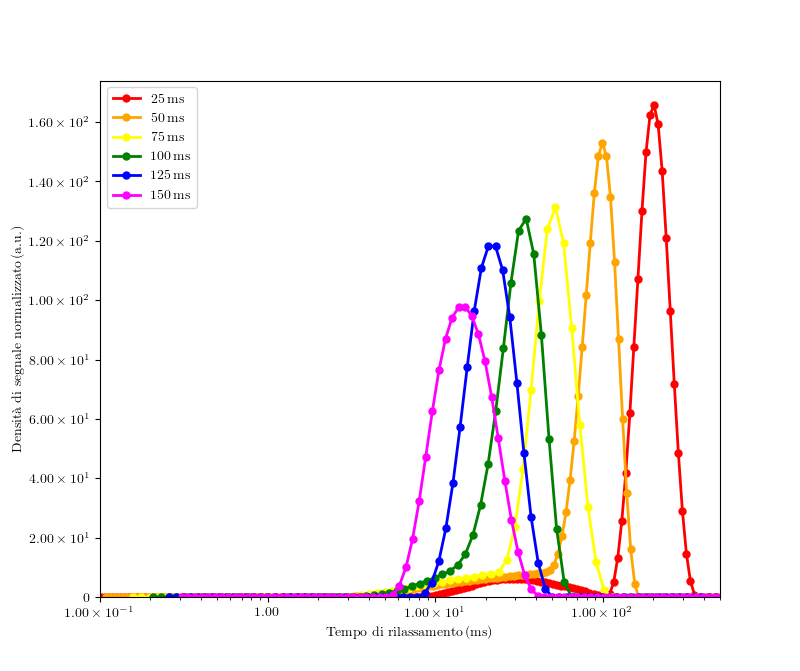
\includegraphics[width=\columnwidth]{Figure/SOLTROL170.png}
\caption{Distribuzioni dei tempi di rilassamento del soltrol 170 per ciascun $\tau$.}
\label{fig:D_s170}
\end{figure}

\begin{figure}[p]
\centering
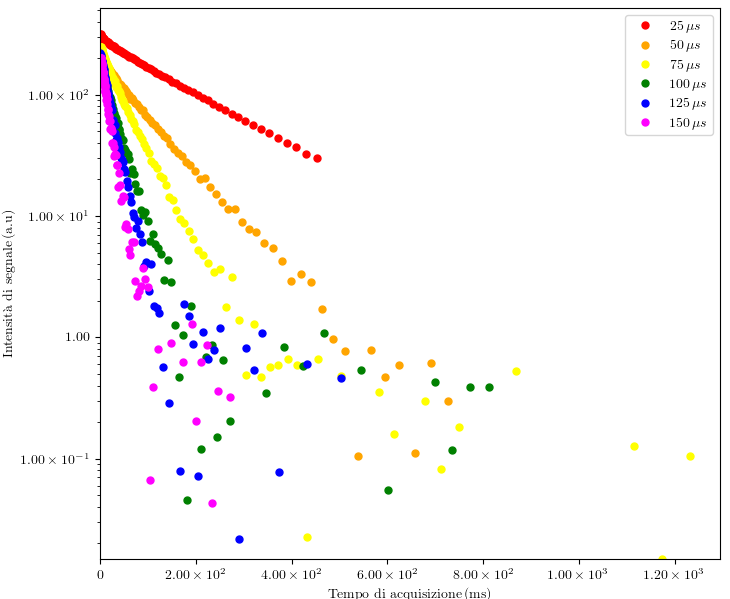
\includegraphics[width=\columnwidth]{Figure/SOLTROL170_SigTSig.png}
\caption{Intensità dei segnali del soltrol 170 per ciascun $\tau$.}
\label{fig:S_s170}
\end{figure}
\newpage Successivamente è stato ricavato il coefficiente di autodiffusione applicando una regressione lineare pesata sui dati di tabella \ref{tab:T_s170}, allo stesso modo che per l'acqua e il soltrol 130.
Il grafico \ref{fig:Df_s170} riporta l'andamento del fit.

\begin{figure}[p]
\centering
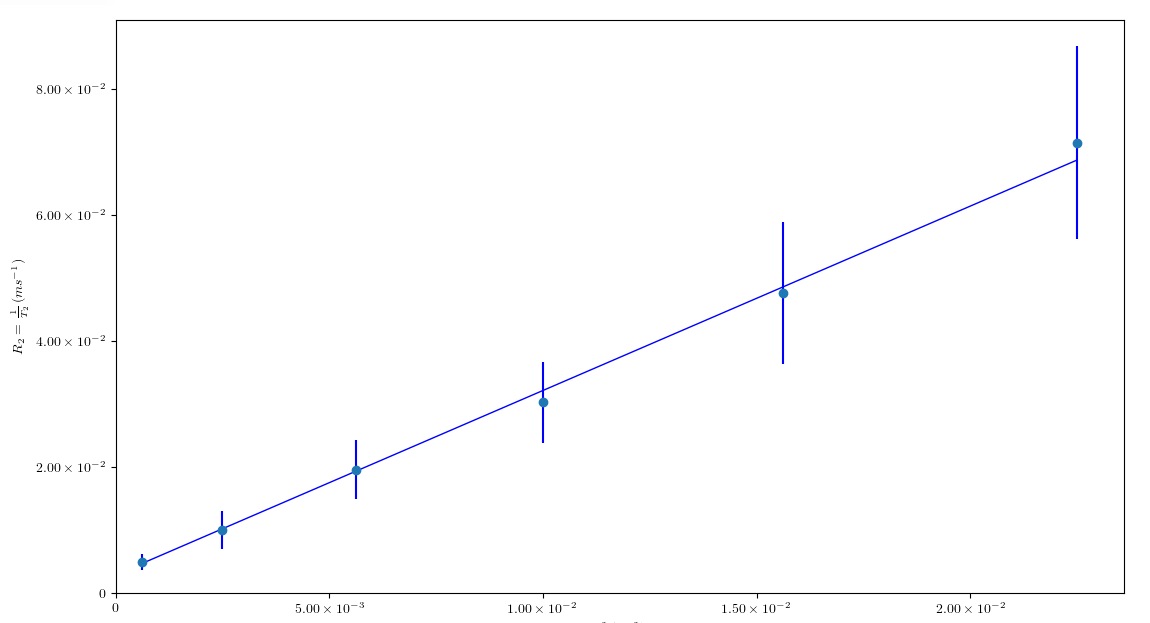
\includegraphics[width=\columnwidth]{Figure/SOLTROL170_calc.png}
\caption{Fit dei dati ottenuti per il SOLTROL 170.}
\label{fig:Df_s170}
\end{figure}
\newpage
Il risultato finale per il coefficiente di autodiffusione del soltrol 170 affetto da errore è contenuto in tabella \ref{tab:T_s170}. 
\begin{table}
    \begin{center}
    \begin{tabular}{c c c}
    \toprule
    	$D\,(\frac{{\mu}^2}{ms})$ & $\sigma\,(\frac{{\mu}^2}{ms})$ \\
    \midrule
    	0.425	&	0.011	\\
    \bottomrule
    \end{tabular}
    \caption{Coefficiente di autodiffusione del soltrol 170 con relativo errore.}
    \label{tab:Df_s170}
    \end{center}
\end{table}




